\chapter{Working Principle}
\setcounter{equation}{0}
\section{URL Input and List Check}
When a user clicks an external link, the browser plug-in captures the destination URL. It first checks whether the domain appears in a trusted allowlist or a known-malicious blocklist. If a domain is already listed, the corresponding classification can be returned without running the machine-learning model. If the domain is not listed, it proceeds to feature extraction and prediction.\cite{bib1}

\section{Feature Extraction}
The research system extracts more than 90 candidate URL and domain characteristics. These include lexical features, DNS and network information, security/authentication signals, domain reputation, and URL behaviour. Examples include URL length, the number of hyphens in the URL path, brand-related keywords, authentication-related keywords in subdomains, nameserver count, the number of dots in the URL, HTTPS presence, and domain registration age. Since feature availability differs between datasets, common features are compared before selecting the final set.\cite{bib1}

\begin{figure}[htbp]
\centering
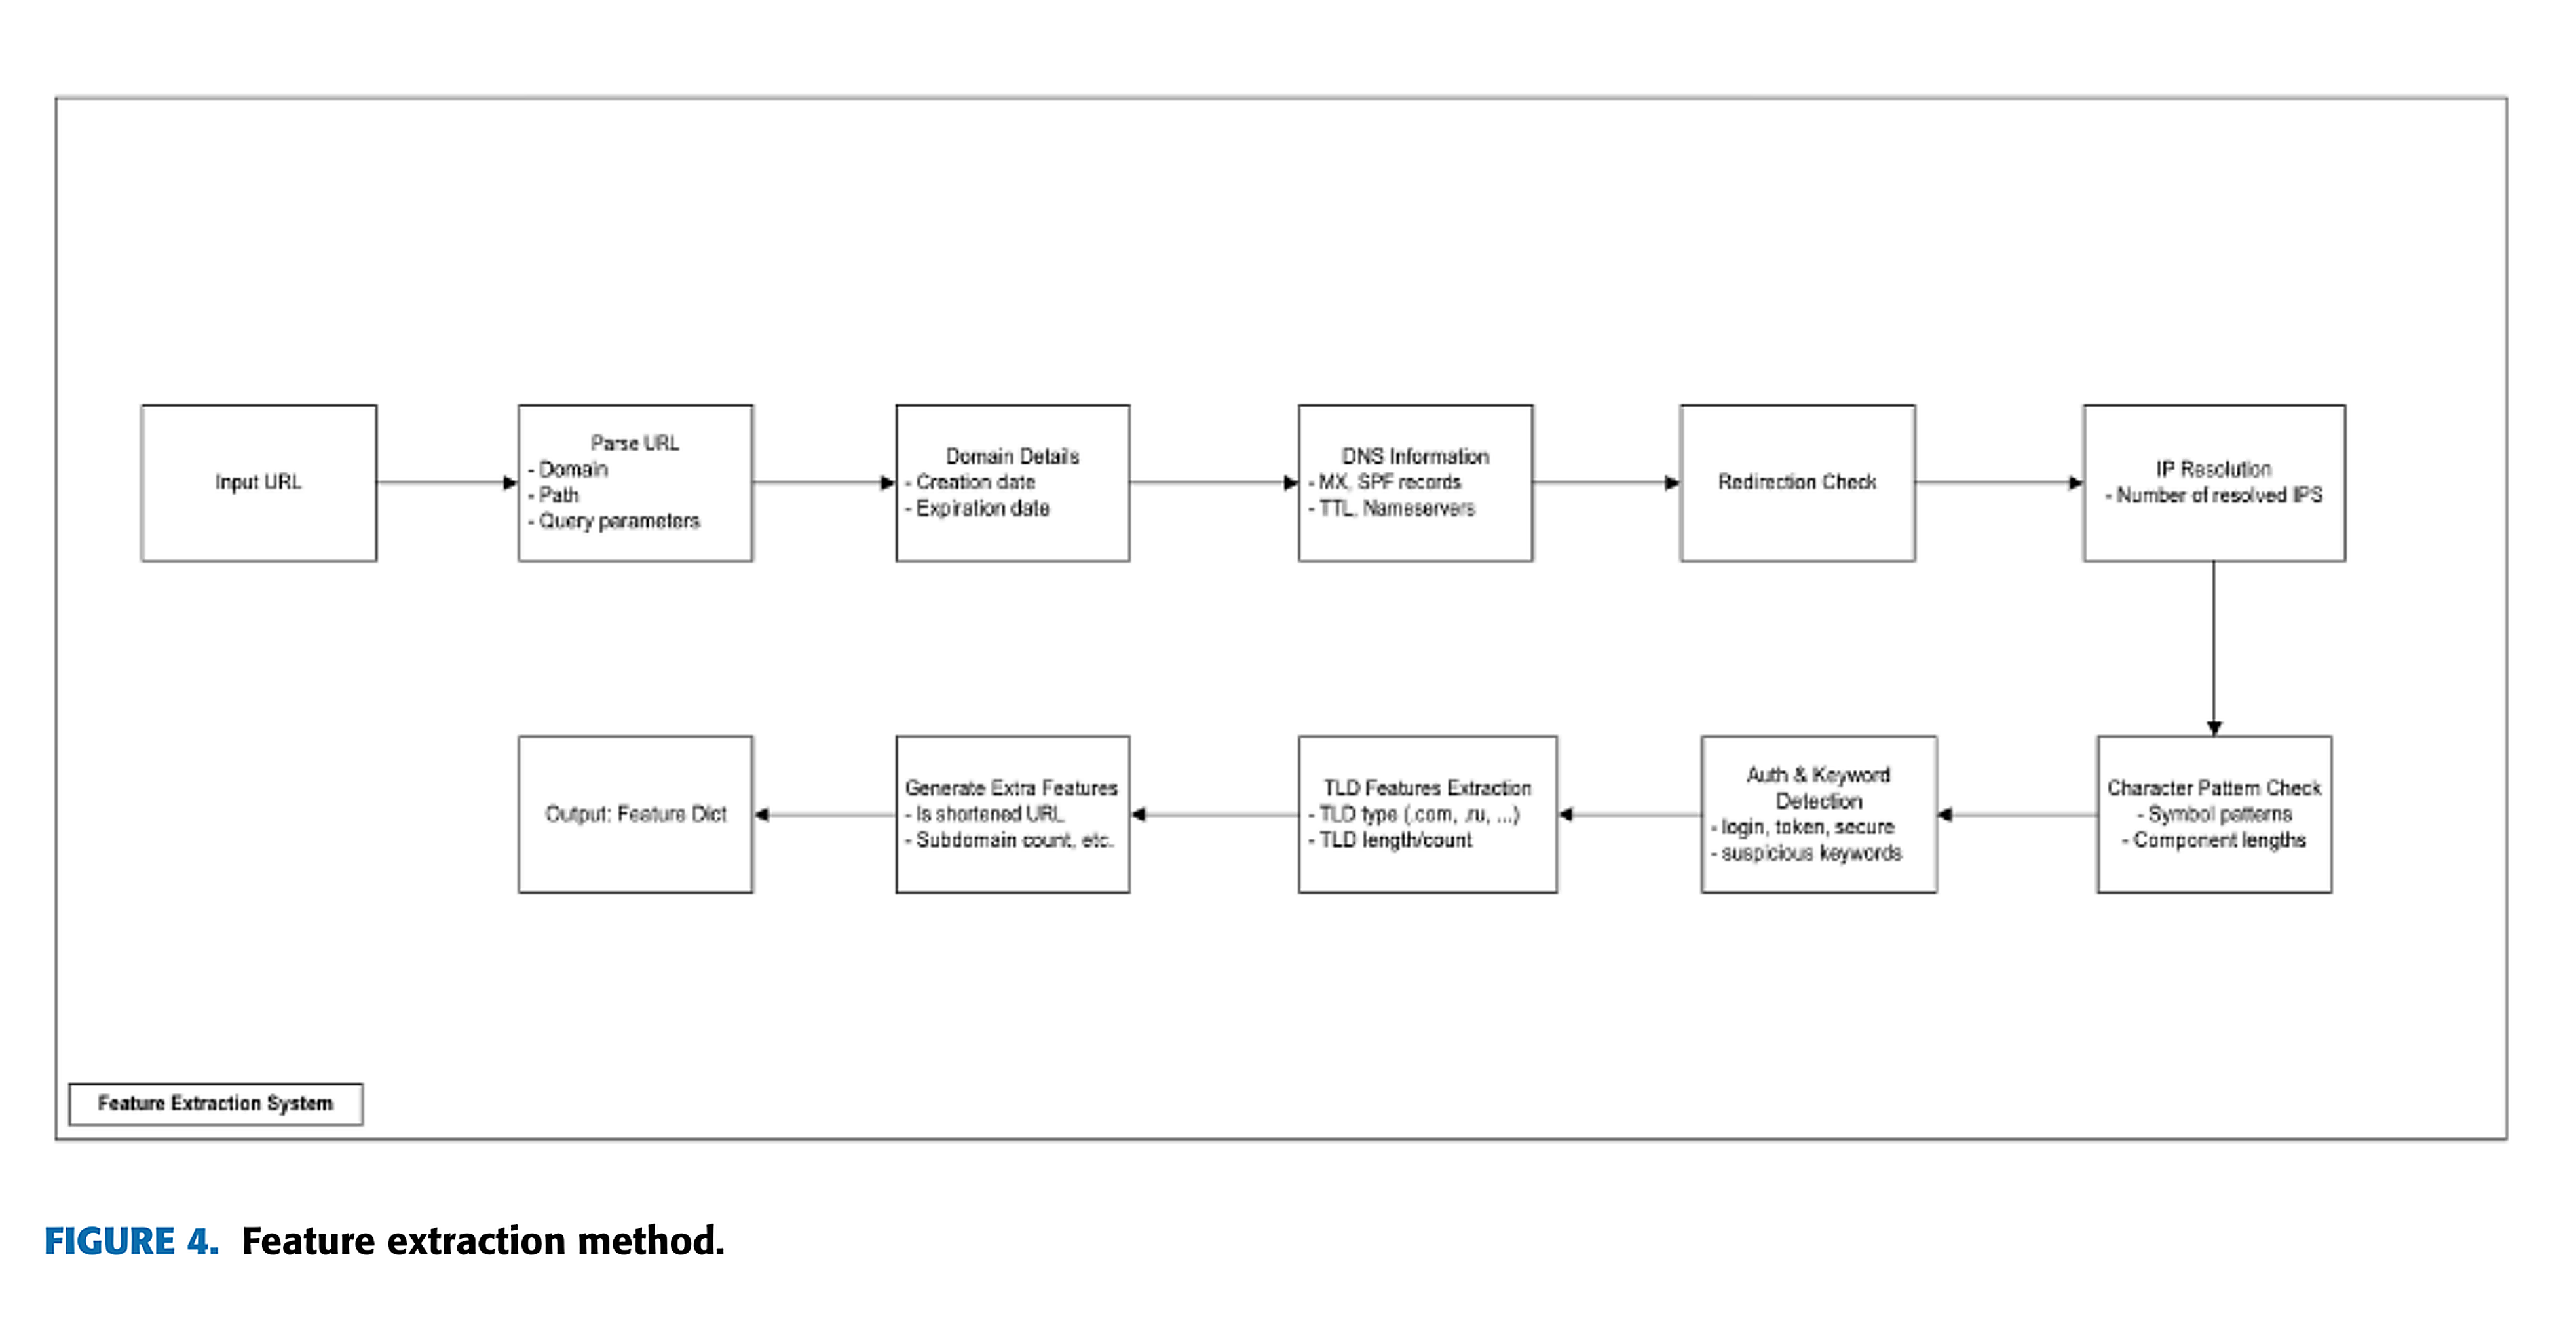
\includegraphics[width=\textwidth,keepaspectratio]{images/pipeline.png}
\caption{Feature extraction pipeline used to construct URL and domain features.}
\label{fig:feature-pipeline}
\end{figure}

\section{Selection of Eight Features}
The authors apply criteria intended to prioritise cross-dataset reliability over performance on one dataset alone: mean importance greater than 0.02, minimum importance greater than 0.005, coefficient of variation below 0.8, and presence in at least 75\% of datasets. The paper notes that only one of 32 analysed features met every criterion, illustrating the difficulty of finding stable signals. The final model uses eight selected features, including URL length, hyphen count in the path, brand-related keywords, authentication-related subdomain count, nameserver count, dot count, HTTPS presence, and domain registration age.\cite{bib1}

\section{Bayesian Hyperparameter Optimisation}
The model's hyperparameters were tuned using BayesSearchCV from scikit-optimize. The search used stratified five-fold cross-validation on the custom dataset, a budget of 100 evaluations, and parallel execution across available CPU cores. The optimisation objective was cross-validated accuracy. The authors then refitted the selected configuration and evaluated it on held-out and independent datasets. Class imbalance was addressed using XGBoost's \texttt{scale\_pos\_weight}, tuned to approximately 1.95.\cite{bib1}

\section{Prediction and Risk Classification}
The trained XGBoost model estimates the probability that a URL is associated with phishing. In the described plug-in workflow, an allowlisted domain is marked safe; a blocklisted domain is marked potentially harmful. For domains not on either list, probabilities below 40\% are labelled safe, values from 40\% to 80\% suspicious, and values above 80\% potentially harmful. The article also reports experimental evaluation at a fixed threshold of 0.85 and threshold selection to meet target specificity levels; these experiment thresholds should not be confused with the user-facing three-category rule.\cite{bib1}

\section{Result Display and Feedback}
The plug-in displays the prediction and risk category to the user. Users can manually confirm a classification, and the domain decision is saved to the corresponding allowlist or blocklist for future checks. This combination of lists and model predictions provides a practical route to real-time URL screening.

\section{Step-by-Step Summary}
\begin{enumerate}
\item Capture the URL when an external link is selected.
\item Check the domain against allowlist and blocklist data.
\item Extract the required URL and domain features if no list entry exists.
\item Apply the selected eight-feature XGBoost model.
\item Convert the prediction into a risk category.
\item Show the classification and allow user feedback.
\item Store confirmed domain classifications for future reference.
\end{enumerate}
